\chapterimage{Preliminary.jpg} % Chapter heading image

\chapter{Preliminary Treatment}

			\begin{itemize}
				\item The objective of preliminary treatment is to remove coarse solids and other large materials often found in raw wastewater
				\item Removal of these materials is necessary to enhance the operation and maintenance of subsequent treatment units\\
				\item Preliminary treatment operations typically include a combination of the following processes:
					\begin{itemize}
						\item Screening
						\item Grinding or shredding
						\item Flow measurement
						\item Grit removal
						\item Pre-aeration
						\item Flow equalization
					\end{itemize}
			\end{itemize}

				
		\section{Process Elements of Preliminary Treatment}\index{Process Elements of Preliminary Treatment}	
			
		\subsection{Screening}\index{Screening}
					\begin{itemize}
						\item Screening is typically the first unit in a preliminary treatment
						\item Screening allows for the capture of coarse solids as pieces of cloths garbage so as to protect pumps and other units from clogging. 
						\item Screens may consist of vertical or inclined bars (bar racks or bar screens), wire mesh or perforated plates having either circular or rectangular openings. 
						\item Screens remove the large, entrained, suspended or floating solids such as pieces of wood, cloth, paper, plastics, garbage, etc.
						\item Debris collected on the screen can be cleaned manually or automatically using chain driven rakes 
						\item The retained material at screens - screenings, is collected and hauled to landfill for disposal
						\item The quantity of screenings removed varies by location and is a function of the clear opening of the screen.
						\item Barmuinitors combine the function of a screen and a grinder.  The ground material is returned to the wastewater flow for removal during primary treatment.
					\end{itemize}

\begin{figure}
\begin{center}
    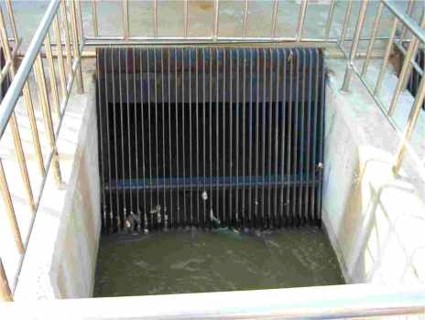
\includegraphics[width=0.7\linewidth]{Barscreen}\\

Barscreen - No rakes
\end{center}
  \end{figure}
  
% \begin{center}
%    
\includegraphics[scale=0.6]{Blank}\\
%\hspace{0cm} Video: Automatic Barscreen
%  \end{center}
 
		\subsection{Grinding and Shredding}\index{Grinding and Shredding}

					\begin{itemize}
\begin{minipage}{\textwidth}	\item Comminutor(Grinder) consist of fixed, rotating or oscillating teeth or blades, acting together to reduce the solids to a size which will pass through fixed or rotating screens grind rags into small chunks
\item The comminutors are installed in wastewater channel and they grind the larger solids without actually removing them from the wastewater.  These devices may be installed before the screens or as a combination of screen and cutters (barmunitors).
					\end{minipage}	
					\end{itemize}
					\begin{minipage}{\textwidth}
					\begin{center}
      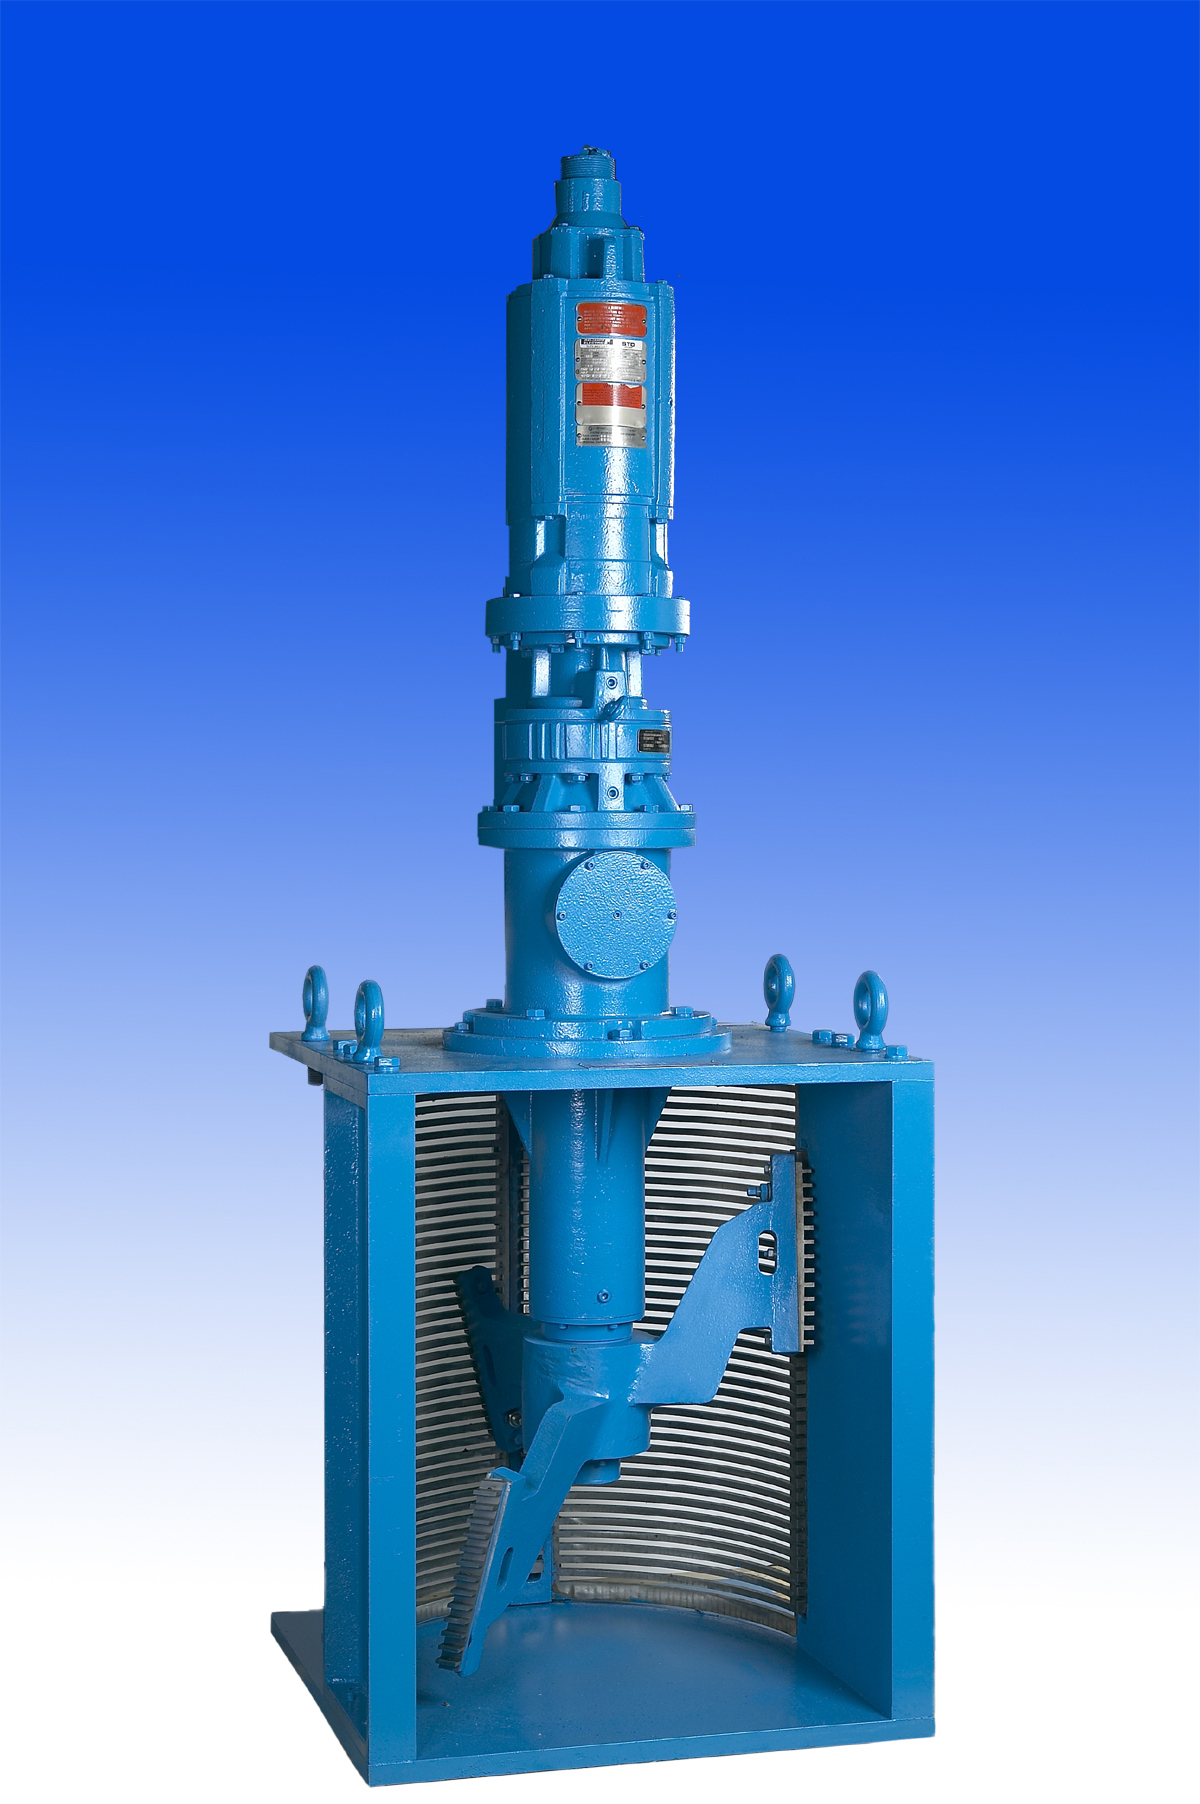
\includegraphics[width=0.3\linewidth, height=70mm]{Comminutor}\\
      Comminutor\\
\end{center}
    \end{minipage}

\begin{figure}[h]
    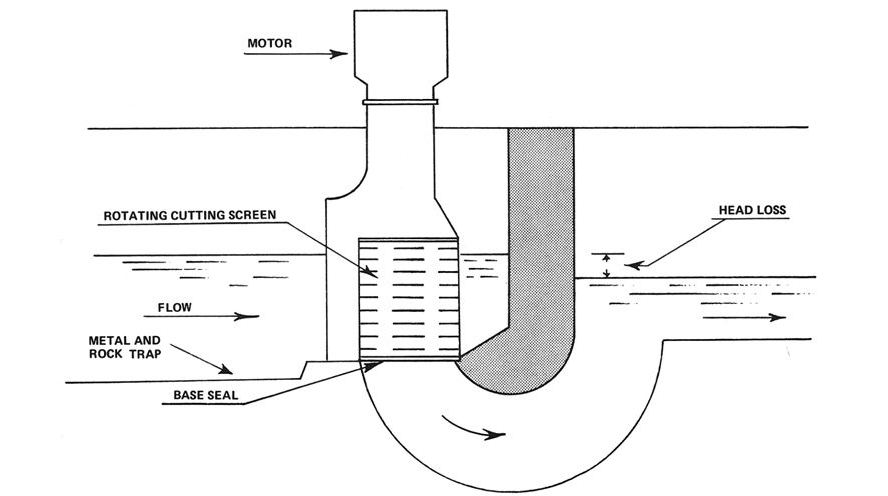
\includegraphics[width=\linewidth]{Comminutor1}\\
    \hspace{5cm}Schematic of comminutor placement in a channel\\
%    \caption{Comminutor Schematic}
  \end{figure}
  
		\subsection{Flow Measurement}\index{Flow Measurement}
					\begin{itemize}
						\item Wastewater flow to a treatment plant is not constant but varies in a diurnal (daily) pattern reflecting domestic water use activity.
						\item Continuous flow measurement is necessary in order to monitor diurnal variations in flow which may affect treatment plant efficiency.\\
						\item Devices used for flow measurement as part of the preliminary treatment can be placed in a channel or in a pipe.
					\end{itemize}

		\subsubsection{Devices for Flow Measurement in Channels}\index{Devices for Flow Measurement in Channels}

					\begin{itemize}
						\item Weirs: 
							\begin{itemize}
								\item Typically sharp crested weirs which are essentially metal plates installed perpendicular the flow.  The plate may a straight edge, a V-notch, or a trapezoidal opening.
								\item The weir plate in the channel causes an increase in the depth of the water behind the weir.  which is proportional to the flow rate.
								\item The flow rate can be determined by calculation or by reading the corresponding flow value to the depth of the water, from a chart specific for that weir. 
								
						
\begin{figure}[h!]
  \centering
  \begin{subfigure}[b]{0.4\linewidth}
    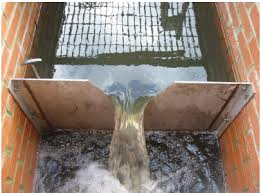
\includegraphics[width=\linewidth]{ChannelWeir}
    \caption{Weir in a channel}
  \end{subfigure}
  \hspace{1cm}
  \begin{subfigure}[b]{0.4\linewidth}
    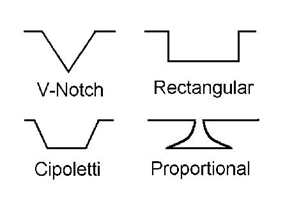
\includegraphics[width=\linewidth]{WierTypes}
    \caption{Weir types}
  \end{subfigure}
\end{figure}
								
								
								
							\end{itemize}
						\item Parshall Flume:
							\begin{itemize}
								\item Parshall flume uses a narrow section in the channel as the restriction rather than the vertical plate of a weir.
								\item Like the weir, the restriction due to the narrow section of the flume, causes an increase in the depth of the water behind the weir (head) which is proportional to the flow rate.
								\item The flow rate can be determined by calculation or by reading the corresponding flow value to the depth of the water, from a chart specific for that Parshall Flume. 
								\end{itemize}

					\end{itemize}
\begin{figure}[h!]
  \centering
  \begin{subfigure}[b]{0.4\linewidth}
    \includegraphics[width=0.75\linewidth]{parshallflume1}
    \caption{Parshall flume}
  \end{subfigure}
  \hspace{1cm}
  \begin{subfigure}[b]{0.4\linewidth}
    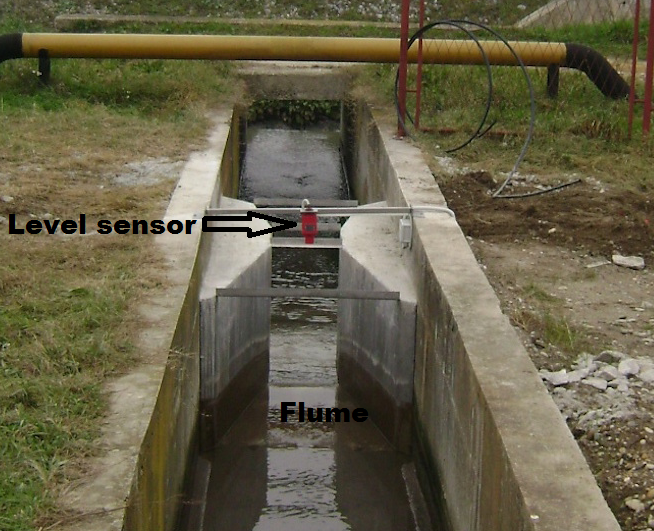
\includegraphics[width=\linewidth]{parshallflume2}
    \caption{Parshall flume with level sensor}
  \end{subfigure}
\end{figure}
		\subsubsection{Devices for Flow Measurement in Pipes}\index{Devices for Flow Measurement in Pipes}
					
					\begin{itemize}
						\item Venturi Tube:
							\begin{itemize}
								\item Measures the difference in pressure in the inlet and center section (throat)
								\item This pressure difference can then be mathematically converted to a flow rate.
								\item Works only when a pipe if flowing full
							\end{itemize}
						\item Magnetic Flow Meter (Magmeter):
							\begin{itemize}
								\item Magmeter is a pipe spool which has an electromagnetic coil surrounding it.  As the wastewater - a conducting material, flows through it, an electrical current is created proportional to the velocity of the conducting fluid (wastewater).
								\item Flow is automatically calculated by multiplying the velocity by the cross- sectional area of the pipe.
								\item Similar to the venturi meter, magmeter will read accurately only if the magmeter section of the pipe is flowing full and the wastewater is flowing through it at a certain minimum velocity.
							\end{itemize}
\begin{figure}[h!]
  \centering
  \begin{subfigure}[b]{0.4\linewidth}
    \includegraphics[width=0.9\linewidth]{magmeter1}
    \caption{Magmeter}
  \end{subfigure}
  \hspace{1cm}
  \begin{subfigure}[b]{0.45\linewidth}
    \includegraphics[width=\linewidth]{magmeter}
    \caption{Piping with magmeters}
  \end{subfigure}
\end{figure} 
					\end{itemize}
		\subsection{Grit Removal}\index{Grit Removal}
						\begin{itemize}
							\item Grit includes sand, gravel, cinder, eggshells, bone chips, seeds, coffee grounds, and large organic particles, such as food waste.
							\item Purpose of Grit removal:
								\begin{itemize} 
									\item to protect mechanical equipment from abrasion and abnormal wear 
									\item to reduce clogging caused by deposition of grit particles in pipes and channels, and 
				\item to prevent loading the treatment plant with inert matter that might interfere with the operation of treatment units such as anaerobic digester and aeration tanks.
			\end{itemize}
		\item Removal of organic material along with the grit is undesirable for two reasons:
			\begin{enumerate}
				\item It causes odor issues, and 
				\item Organic matter is a potential source of energy (digester gas)
			\end{enumerate}
		\item Grit Disposal: Grit removed is typically landfilled.
		\item Grit Volume:  The volume of grit collected measured in ft$^3$/MG.
		\item The rate of grit collection can range from 0.5 ft$^3$/MG to 30 ft$^3$/MG.
		\item Wastewater plants having a combined collection system must deal with much larger volumes of grit.
\end{itemize}
\subsubsection{Grit Removal Systems}\index{Grit Removal Systems}



			\begin{itemize}
			
					\item \noindent\textsc{Horizontal grit chambers:}

					\begin{itemize}
						\item These are rectangular channels 30 to 60 feet long and the water detention time is between 45 to 90 seconds
						\item Water passing through these channels is maintained at a relatively constant \hl{velocity of about 1 feet per second (fps)} which allows for the grit to settle while keeping the lighter organic material to stay in suspension and continue on into the primary clarifiers.
					\end{itemize}
	

						\item \noindent\textsc{Aerated grit chambers:}
	
					\begin{itemize}
						\item The 1 fps velocity is maintained by using aerators to create a rolling flow in the tank.
						\item Aeration is achieved using diffusers located on the bottom of one side of the grit chamber.
						\item Aerated grit chambers help create aerobic conditions in septic sewage. Aerobic conditions help improve the settleability of the sludge and increase both BOD and suspended solids removal in the primary clarifiers.
						\item Much larger and deeper than non-aerated units.
						\item The detention times are increased to 3 to 5 minutes.
					\end{itemize}

\begin{figure}[h!]
  \centering
  \begin{subfigure}[b]{0.46\linewidth}
    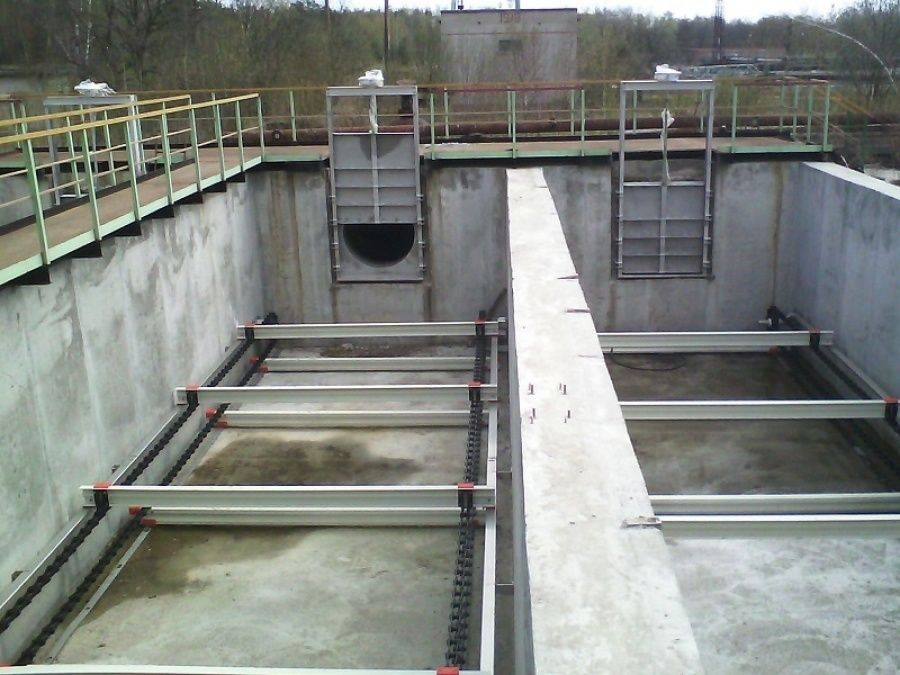
\includegraphics[width=0.8\linewidth]{HorizontalGritChamber}
    \caption{Horizontal grit chamber}
  \end{subfigure}
  \hspace{0.2cm}
  \begin{subfigure}[b]{0.5\linewidth}
    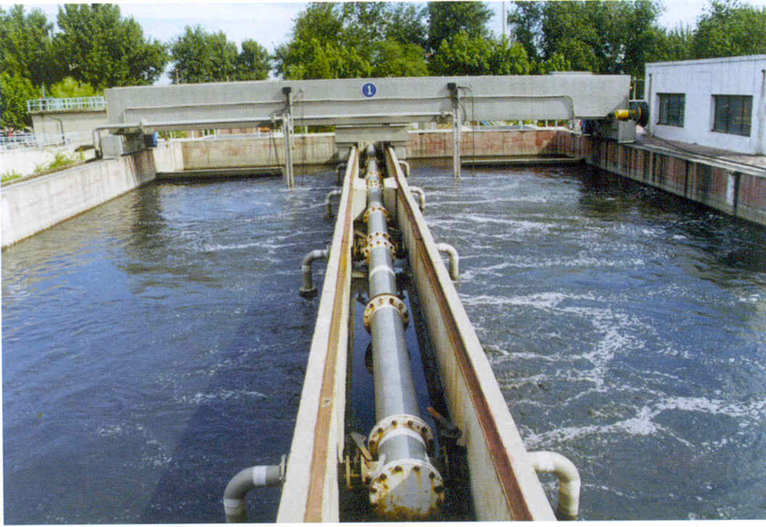
\includegraphics[width=0.8\linewidth]{AeratedGritChamber}
    \caption{Aerated grit chamber}
  \end{subfigure}
\end{figure} 					


						\item \noindent\textsc{Cyclonic/Vortex grit chamber:}


					\begin{itemize}
						\item The wastewater flows into a cylinder that tapers to a cone at one end.
						\item The flow whirls around the inside of the cylinder like a cyclone which causes the heavy grit to be slinged to the outside and it ultimately settles to the bottom from where it is withdrawn.
					\end{itemize}

\begin{figure}[h!]
  \centering
  \begin{subfigure}[b]{0.47\linewidth}
    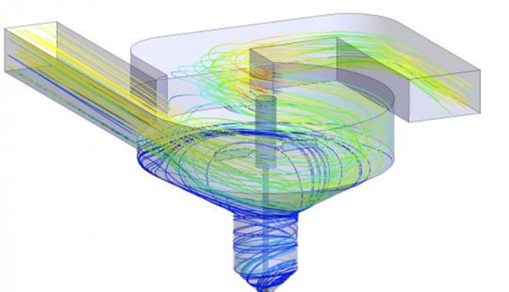
\includegraphics[width=0.8\linewidth]{VortexGritChamber1}
    \caption{Vortex grit chamber design}
  \end{subfigure}
  \hspace{0.2cm}
  \begin{subfigure}[b]{0.43\linewidth}
    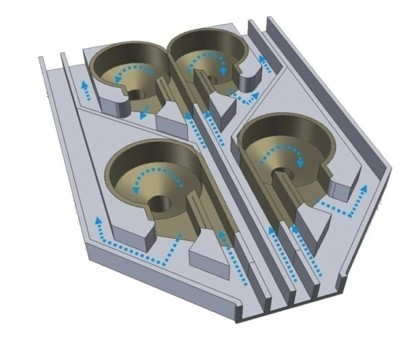
\includegraphics[width=0.8\linewidth]{VortexGritChamber}
    \caption{Vortex grit chamber installed}
  \end{subfigure}
\end{figure} 
	
\subsubsection{Grit Removal}\index{Grit Removal}		

		
			\begin{itemize}
				\item In the cyclonic/vortex grit chamber, the grit is scoured with water and is removed using pumps
				\item For the horizontal and aerated grit systems:
					\begin{itemize}
						\item Mechanical augers at the bottom of the grit chamber move the grit to one end of the tank where grit slurry pumps can pump it out of the tank to a grit separator.
						\item In some cases steep bottom slope is provided which will collect the grit at Central Point of Removal.
						\item Grit Removal is achieved by air pumps for small aerated grit chambers.
						\item Grit can also be removed by tubular conveyors, buckets type collectors, elevators screws conveyors, grit pumps and clam shell buckets
					\end{itemize}
			\end{itemize}
						\end{itemize}
%		\end{itemize}

\subsection{Flow Control}\index{Flow Control}	
	\begin{itemize} 
		\item Flow control is critical for grit removal, specifically for the horizontal and aerated grit chambers as excessive or inadequate velocities would lead to poor grit removal or cause excessive organic material settling along with the grit, respectively
		\item As the wastewater flows vary diurnally, it is important that velocity of the wastewater in the grit chamber should be maintained nearly constant - near 1 fps.
		
\begin{figure}[h]
    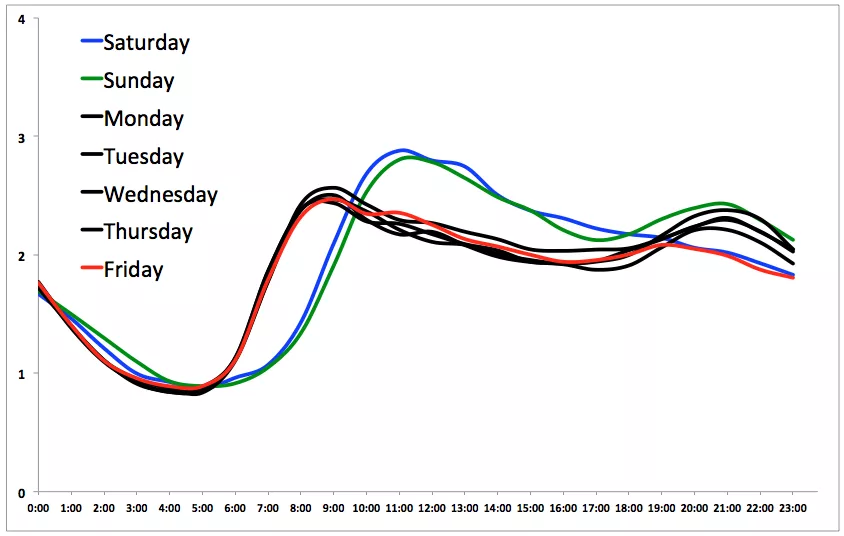
\includegraphics[width=\linewidth]{DiurnalFlow}\\
\begin{center}
Diurnal wastewater flow profile \\
\end{center}
%    \caption{Comminutor Schematic}
  \end{figure}		

		\item Constant velocity in a grit chamber is achieved by providing a \hl{proportional (Sutro) weir} at the outlet end of grit chamber.
		\item The shape of the opening between the plates of a proportional weir is made in such a way that the discharge is directly proportional to liquid depth in grit chamber resulting in maintaining a constant velocity of water even a the flow changes.
	\end{itemize}
\begin{figure}[h!]
  \centering
  \begin{subfigure}[b]{0.5\linewidth}
    \includegraphics[width=0.8\linewidth]{Sutroweir1}
    \caption{Proportional weir design}
  \end{subfigure}
  \hspace{1cm}
  \begin{subfigure}[b]{0.35\linewidth}
    \includegraphics[width=0.8\linewidth]{Sutroweir}
    \caption{Installed Proportional weir}
  \end{subfigure}
\end{figure} 

\subsection{Pre-aeration}\index{Pre-aeration}	
	\begin{itemize}
		\item Pre-aeration of the wastewater as part of the preliminary treatment may be provided as a separate process or increased detention time in an aerated grit chamber.
		\item Pre-aeration provides the follwoing benefits:
			\begin{itemize}
				\item freshens up wastewater by dissolving oxygen thereby reducing the wastewater septicity
				\item reduction of septicity allows for better settling - solids and BOD removal, in the following primary treatment process
				\item promotes grease separation which facilitates its removal during primary treatment
			\end{itemize}
	\end{itemize}
\subsection{Flow Equalization}\index{Flow Equalization}	

	\begin{itemize}
		\item Flow equalization involves storing a portion of peak flows for release during low-flow periods
		\item It prevents surges and allows for the operation of processes at design flows thus allowing for optimal physical, biological and chemical processes to take place.
		\item It results in saving capital costs as the processes may be built with a treatment capacity which is less than the peak flows
	\end{itemize}


\newpage
\section*{Chapter Assessment}
\begin{tcolorbox}[breakable, enhanced,
colframe=blue!25,
colback=blue!10,
coltitle=blue!20!black,  
title= Chapter Assessment]

\begin{enumerate}

\item A weir can be also be used for measuring flows\\

a. True \\
b. False 
\vspace{0.4cm}
\item The process of pre-aeration in no way influences the degree of settling in a primary clarifier\\
\vspace{0.4cm}
a. True \\
b. False 
\vspace{0.4cm}
\item Septic sludge has a low pH\\

a. True \\
b. False 
\vspace{0.4cm}
\item A Parshall flume measures the velocity of the influent flow\\

a. True \\
b. False 
\vspace{0.4cm}
\item  A barminutor frequently operates automatically. \\

a. True \\
b. False 

\vspace{0.4cm}
\item  A grit chamber with a faster flow velocity than recommended may allow appreciable organic matter to collect in the grit. \\

a. True \\
b. False 

\item Carryover of grit from the grit chamber may indicate the need to: \\

a. Increase rate of settled grit removal from the grit chamber.. \\
b. Decrease the operational depth of the channel. \\
c. Increase the flow to the primary clarifier. \\
d. Increase the air input to an aerated grit chamber. 

\vspace{0.4cm}
\item Characteristics that should be measured immediately after the sample is collected are: \\

a. Velocity and dissolved solids \\
b. Temperature, pH and DO \\
c. TSS and BOD \\
d. Hardness and alkalinity 

\vspace{0.4cm}
\item Flow proportionate composite samples are collected because: \\

a. The waste characteristics are continually changing \\
b. The flow is continually changing \\
c. The flow and waste characteristics are continually changing \\
d. This requires less time than grab samples \\
e. All of the above 

\vspace{0.4cm}
\item Grab samples are considered to be representative of the \\

a. Average daily condition at the sample location \\
b. Average daily condition in the system \\
c. System conditions for the two hours before and after the sample was taken \\
d. System condition at the time of the sample 

\vspace{0.4cm}
\item Grit is composed mostly of which of the following substances? \\

a. Grease \\
b. Colloidal solids \\
c. Rubber goods \\
d. Inorganics \\
e. Plastics 

\vspace{0.4cm}
\item Organisms in wastewater that are not harmful to humans but are indicators of diseases are: \\

a. Pathogens \\
b. Viruses \\
c. Coliform \\
d. Bacteria 

\vspace{0.4cm}
\item Which of the following pollutants would be removed to the extent in an efficiently operating grit chamber? \\

a. Egg shells \\
b. Seeds \\
c. Oils and grease \\
d. Sand \\
e. Fixed solids 

\vspace{0.4cm}
\item Proportional weirs usually are located at: \\

a. Immediately after the barscreens \\
b. Primary clarifiers \\
c. Aerobic digester scum boxes \\
d. Grit chambers \\
e. Inside the Parshall flume 

\vspace{0.4cm}
\item Which of the following process units is not usually considered to be a preliminary treatment unit? \\

a. Grit chamber \\
b. Bar screen \\
c. Comminutor \\
d. Bar rack \\
e. A meniscus 

\vspace{0.4cm}
\item  Which of the following would be included in the pretreatment unit? \\

a. preaeration \\
b. grit removal \\
c. screening \\
d. comminutor \\
e. all of the above 

\end{enumerate}
\end{tcolorbox}







